% this file is called up by thesis.tex
% content in this file will be fed into the main document

%: ----------------------- name of chapter  -------------------------
\chapter{Projekt i implementacja} % top level followed by section, subsection


%: ----------------------- paths to graphics ------------------------

% change according to folder and file names
\ifpdf
    \graphicspath{{6/figures/PNG/}{6/figures/PDF/}{6/figures/}}
\else
    \graphicspath{{6/figures/EPS/}{6/figures/}}
\fi

%: ----------------------- contents from here ------------------------

Rozdział ten opisuje architekturę, projekt i implementację przykładowej platformy integracyjnej zwanej dalej SpeechProcessingPlatform, która umożliwi weryfikację proponowanego podejścia. Platforma ta jest projektowana z myślą o architekturze opartej na technologii ESB, którą autorzy uznali za najlepiej nadającą się do realizacji systemów integracyjnych. Rozdział ten zawiera opis najważniejszych części systemu, zależności między nimi oraz format danych wykorzystywanego w komunikacji.

\section{Architektura}

Rysunek \ref{fig:layered_architecture} przedstawia architekturę systemu SpeechProcessingPlatform. Jest ona podzielona na 3 warstwy:

\begin{itemize}
	\item Data Endpoints Layer
	\item Routing Layer
	\item Services Layer
\end{itemize}

\begin{figure}[!h]
	\centering
	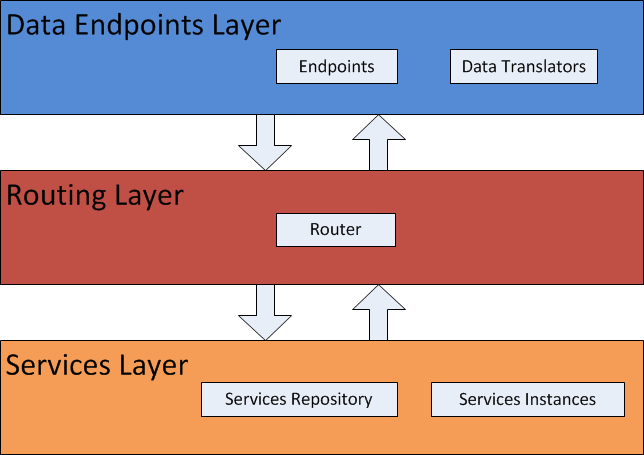
\includegraphics[scale=0.7]{layered_architecture.png}
	\caption{Architektura systemu SpeechProcessingPlatform}\label{fig:layered_architecture}
\end{figure}

Podejście warstwowe ułatwia dekompozycję systemu na niezależne komponenty, które odpowiadają za dobrze zdefiniowany fragment wymaganej funkcjonalności. 
% tu mozna cos dodac jak cos

Warstwa \textit{Data Endpoints Layer} odpowiada za udostępnianie interfejsów dla aplikacji klienckich oraz za transformacje danych do wspólnego formatu. Głównymi elementami tej warstwy są endpointy i translatory danych. Endpointy wystawiają interfejsy umożliwiające dostęp do platformy przy użyciu różnych technologii takich jak REST, FTP, SOAP czy RSS. Zadaniem translatorów jest ujednolicenie danych do postaci używanej w kolejnych warstwach. Dzięki temu komponenty z warstw niższych mają uproszczoną implementację ponieważ skupiają się na obsłudze tylko jednego, dobrze zdefiniowanego formatu. 

Warstwa \textit{Routing Layer} odpowiada za routowanie zadań przetwarzania od endpointów to odpowiednich serwisów, a także za przesyłanie wyników z powrotem do endpointów. Zadania mogą być jedno etapowe jak np. \textit{przetłumacz ten tekst z języka polskiego na język angielski} albo dwu lub więcej etapowe jak np. \textit{rozpoznaj tekst na tym zdjęciu, jeżeli trzeba przetłumacz na język angielski i na jego podstawie wygeneruj dźwięk}.

Głównym elementami ostatniej warstwy, \textit{Services Layer}, jest repozytorium serwisów oraz konkretne ich instancje. Główne zadanie repozytorium to wyszukiwanie i zwracanie odpowiednich instancji w odpowiedzi na żądania warstwy routującej. Najważniejszą cechą wyróżniającą poszczególne serwisy jest typ przetwarzania mowy jaki dostarczają. Wyróżniamy 5 typów serwisów, a każdy z nich posiada dodatkowe cechy, które także mają wpływ na wynik wyszukiwania:

\begin{itemize}
	\item OCR
	\begin{itemize}
		\item obsługiwane formaty zdjęć
	\end{itemize}
	\item ASR
	\begin{itemize}
		\item obsługiwane języki 
		\item obsługiwane formaty wejściowe
	\end{itemize}
	\item TTS
	\begin{itemize}
		\item obsługiwane języki 
		\item obsługiwane formaty wyjściowe
	\end{itemize}
	\item translacja
	\begin{itemize}
		\item obsługiwane języki
	\end{itemize}
	\item rozpoznawanie języka
\end{itemize}

Oczywiście konkretny serwis może udostępniać więcej niż jeden typ przetwarzania np. serwis translacji może od razu być w stanie rozpoznać język źródłowy, dzięki czemu nie musi mieć tej informacji dostarczonej razem z tekstem.

\begin{figure}[!h]
	\centering
	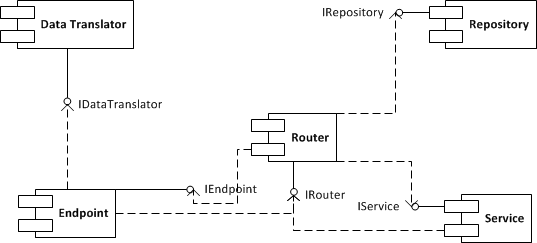
\includegraphics[scale=1.0]{component_uml.png}
	\caption{Diagram komponentów systemu SpeechProcessingPlatform w notacji UML 1.0}\label{fig:component_diagram}
\end{figure}

\section{Projekt}

Jak było wspomniane, do realizacji systemu SpeechProcessingPlatform została wybrana technologia ESB. Głównymi zaletami tej technologii są skalowalność i wysoki poziom abstrakcji, dzięki któremu budowa systemu jest ułatwiona - pozwala skupić się na problemie a nie na szczegółach implementacji. Dodatkowo, kontenery ESB dostarczają dużo użytecznych funkcjonalności takich jak: routing, transformacja danych, komunikacja oparta na wiadomościach, zestaw gotowych endpointów dzięki którym integracja jest znacznie prostsza. Projektowanie systemu z użyciem wiadomości jako modelu komunikacji, różni się od tradycyjnego podejścia z blokującym wywołaniem metod. Interfejsy w postaci listy pól i metod, które dany komponent implementuje zostają zastąpione przez odpowiednie kanały wiadomości oraz format danych, które będą nimi przesyłane. Dzięki użyciu tego modelu, zastosowanie dobrze sprawdzonych wzorców EIP staję się bardzo naturalne. 

\subsection{Warstwa \textit{Data Endpoints Layer}}

Ilustracja \ref{fig:endpoins_layer_project} przedstawia przepływ wiadomości w warstwie \textit{Data Endpoints Layer}. Aplikacje klienckie wysyłają żądanie przetwarzania na określony endpoint, używając wybranego i obsługiwanego przez platformę protokołu. Żądania te zostają przetłumaczone na wspólny format wiadomości używany w dalszych częściach systemu, a następnie przesłane do routera. Dodatkowo, każdy punk końcowy posiada swój indywidualny kanał odpowiedzi, którego adres jest dodawany do wiadomości jako adres zwrotny. Dzięki temu, router będzie wstanie odesłać wynik przetwarzania do odpowiedniego endpointu.

\begin{figure}[!h]
	\centering
	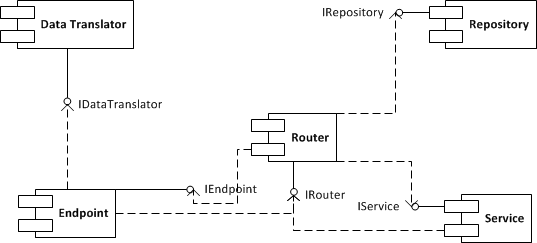
\includegraphics[scale=1.0]{component_uml.png}
	\caption{MOCK Diagram przepływu wiadomości w warstwie \textit{Data Endpoints Layer}}\label{fig:endpoins_layer_project}
\end{figure}

Ponieważ przetwarzanie mowy może być procesem czasochłonnym, budowana platforma powinna wspierać komunikację asynchroniczną, która umożliwi uniknięcie zbędnego oczekiwania na odpowiedź. Niektóre punkty końcowe, takie jak FTP czy SMTP są z natury asynchroniczne. Aplikacja wykorzystująca protokół SMTP wysyła emaila z wymaganymi załącznikami na adres endpointa i wraca do swojego przetwarzania. Email zostaje odebrany przez platformę, następuje proces przetwarzania, a odpowiedź jest odsyłana na adres nadawcy. Gdy aplikacją odbierze emaila zwrotnego może zacząć przetwarzanie odpowiedzi w dogodnym dla siebie czasie. Inne końcówki, takie jak REST czy SOAP, posiadają naturę synchroniczną, dlatego aby wspierały one komunikację asynchroniczną należy zastosować dodatkowe mechanizmy. W wybranym przez autorów rozwiązaniu większość odpowiedzialności za dodanie obsługi asynchronicznej komunikacji spada na kolejne warstwy. Jedynym dodatkowym zadaniem punktów końcowych jest oznaczenie wiadomości jako przeznaczonej do przetwarzania asynchronicznego. Przy takim oznaczeniu, odpowiedź z warstwy routującej przychodzi bardzo szybko, lecz zawiera ona tylko identyfikator odpowiedzi, dzięki któremu aplikacja kliencka będzie mogła odpytać system czy jej zadanie zostało już zakończone. Takie zapytanie jest jest traktowane w taki sam sposób jak żądanie przetwarzania. Jeżeli zadanie zostało zakończone, wynik zostanie zwrócony aplikacji. Jeżeli nie, aplikacja będzie musiała wykonać zapytanie ponownie.

\subsection{Warstwa \textit{Routing Layer}}

\subsection{Warstwa \textit{Services Layer}}


%Jednym z rozwiązań jest użycie wzorca \textit{Correlation Identifier}\cite{eaipatterns}:

%\begin{figure}[!h]
%	\centering
%	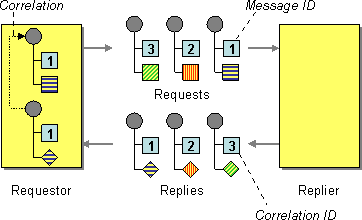
\includegraphics{CorrelationIdentifierSolution.png}
%	\caption{Wzorzec \textit{Correlation Identifier}: \url{http://www.eaipatterns.com/img/CorrelationIdentifierSolution.gif}}\label{fig:correlation_identifier}
%\end{figure}

%Endpoint po otrzymaniu żądania generuje dla niego unikalny identyfikator, który odsyła aplikacji nie czekając na wynik przetwarzania. Ten sam identyfikator jest dodawany do wiadomości %wysyłanej do routera, lecz tym razem adres zwrotny wskazuje nie na endpoint lecz na serwis 



% rysunek z podziałęm na komponenty,
% rysunek EIP - ale to może być już w projekcie.
% proekt, interfejsy, chierarchie klas. 









% ---------------------------------------------------------------------------
%: ----------------------- end of thesis sub-document ------------------------
% ---------------------------------------------------------------------------

